\documentclass[dvipdfmx]{standalone}
\usepackage{tikz}

\usetikzlibrary{
  arrows.meta,
  positioning,
  shapes.geometric,
  calc,
  fit,
  backgrounds,
  decorations.pathreplacing,
  decorations.pathmorphing,
  decorations.markings,
  patterns,
  matrix,
  shapes.multipart
}

\begin{document}

\begin{tikzpicture}
  \def\y{3}

  \node (A) at (0,+1.0*\y) {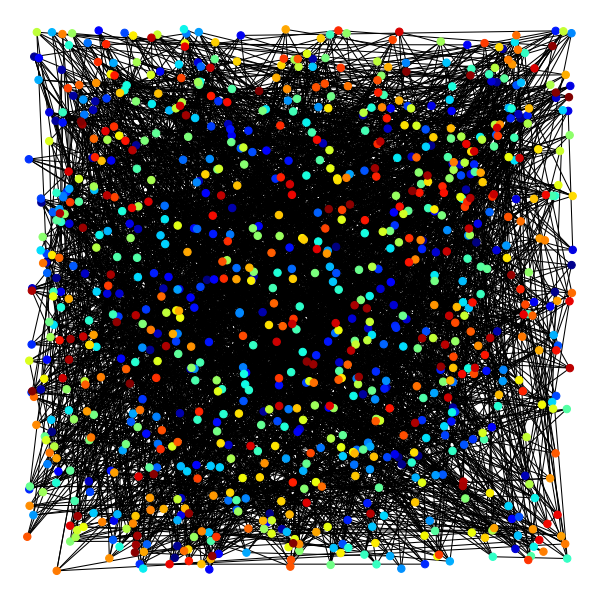
\includegraphics[width=3cm]{../individual/vis/fig1_init_random.png}};
  \node[above=0.1cm of A, scale=1.2] {\large{\textsf{random}}};

  \node (B) at (+6, +1.5*\y) {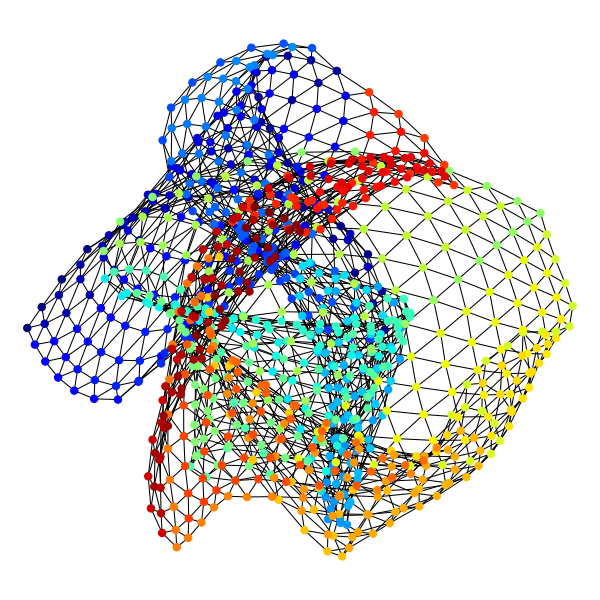
\includegraphics[width=3cm]{../individual/vis/fig1_jagmesh1_FR.png}};

  \node (C) at (+6, +0.5*\y) {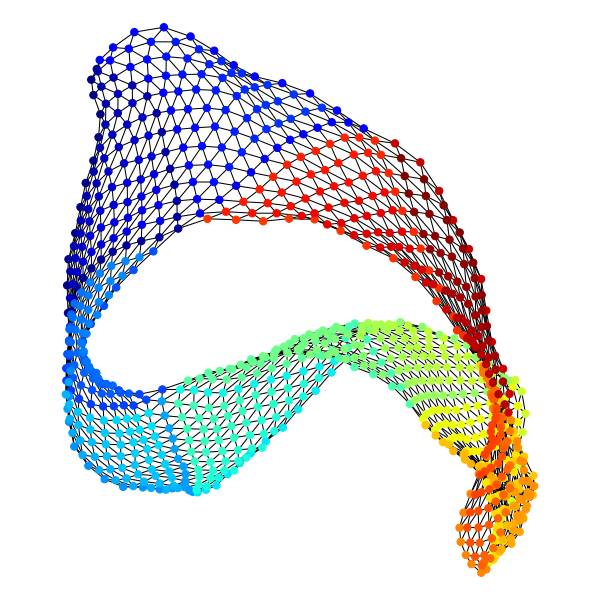
\includegraphics[width=3cm]{../individual/vis/fig1_jagmesh1_L-BFGS.png}};

  \node (D) at (0, -1.0*\y) {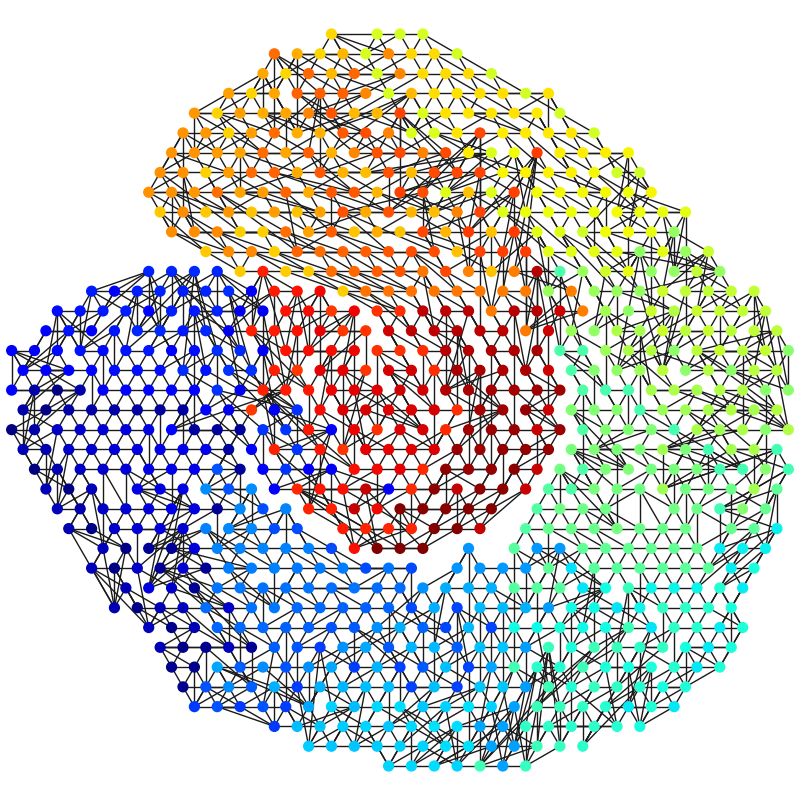
\includegraphics[width=3cm]{../individual/vis/fig1_init_CN.png}};

  \node (E) at (+6, -0.5*\y) {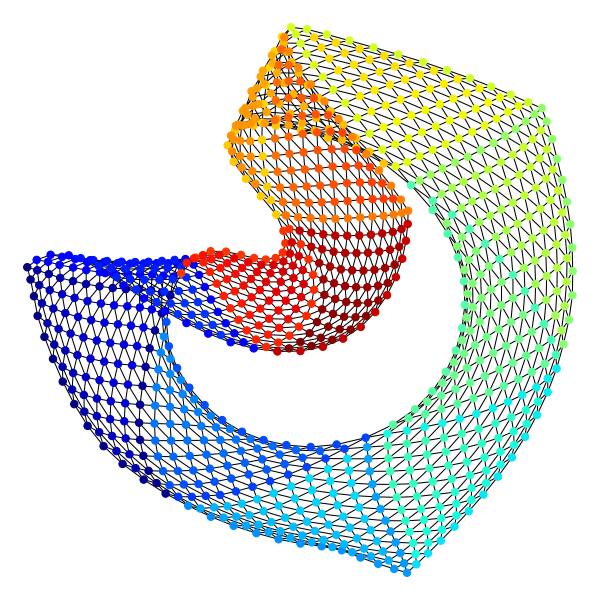
\includegraphics[width=3cm]{../individual/vis/fig1_jagmesh1_CN-FR.png}};

  \node (F) at (+6, -1.5*\y) {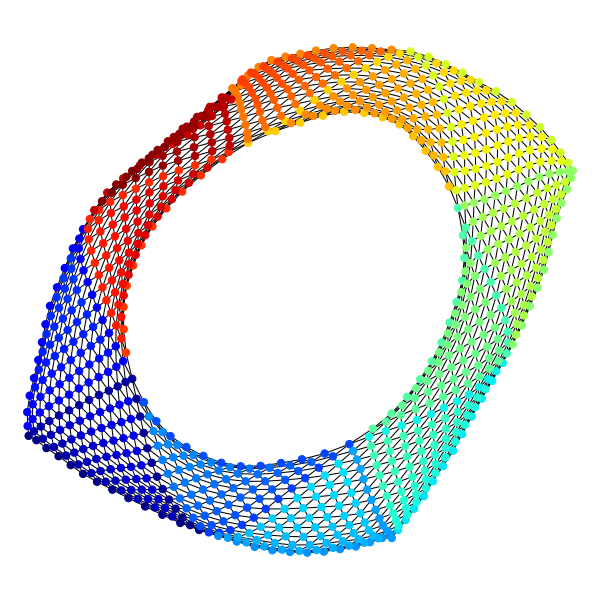
\includegraphics[width=3cm]{../individual/vis/fig1_jagmesh1_CN-L-BFGS.png}};

  % Draw arrows with labels
  \draw[-{Stealth[length=2mm,width=3mm]},line width=0.07cm] (A) -- (B) node[midway, above=0.4cm,scale=1.2] {\Large{\textsf{FR}}};
  \draw[-{Stealth[length=2mm,width=3mm]},line width=0.07cm] (A) -- (C) node[midway, below=0.4cm,scale=1.2] {\Large{\textsf{L-BFGS}}};
  \draw[-{Stealth[length=3mm,width=4mm]},line width=0.1cm, red] (A) -- (D) node[midway, right, red,scale=1.2] {\LARGE{\textbf{\textsf{proposed}}}};
  \draw[-{Stealth[length=2mm,width=3mm]},line width=0.07cm] (D) -- (E) node[midway, above=0.4cm,scale=1.2] {\Large{\textsf{FR}}};
  \draw[-{Stealth[length=2mm,width=3mm]},line width=0.07cm] (D) -- (F) node[midway, below=0.4cm,scale=1.2] {\Large{\textsf{L-BFGS}}};

\end{tikzpicture}

\end{document}
